
\subsection{Historical review}
%% Problèmes traités -- approche expérimentale pour la confirmation
%% Type de solutions
%% Simple waves even for linear hardening in contrast to one-dimensional problems

\begin{frame}{Thin-walled tube problem}%{Historical review}
  \begin{columns}
    \begin{column}{0.4\textwidth}
      \begin{block}{\footnotesize Semi-infinite medium}
        % \centering
        \begin{tikzpicture}
          \begin{scope}[shift={(-1.75,0)}]
            \draw[->] (0,0) -- (0.5,0) node[right] {\scriptsize $x_1$};
            \draw[->] (0,0) -- (0,0.5) node[above] {\scriptsize $x_2$};
          \end{scope}
          \draw (0,0) -- (3,.0);
          \draw[very thick] (0,0) -- (0,2.);
          \fill [pattern=north east lines] (0,0) rectangle (3.,2.);
          \draw[dash dot] (-0.5,0) -- (3.5,0);% node[right] {\footnotesize $x_1$};
          % \draw[->,dash dot] (0,0) -- (0,2.5) node[above] {\footnotesize $x_2$};
          \foreach \y in {0,0.25,...,1.75}
          \draw[Red,->,>=stealth] (-0.1,\y) -- (-0.1,\y+0.15);
          \foreach \y in {0,0.25,...,1.75}
          \draw[Red,->,>=stealth] (-0.30,\y+0.20) -- (-0.15,\y+0.20);
          \node[Red,left] at (-0.3,1.) {\scriptsize $\sigma,\tau$};
        \end{tikzpicture}  
      \end{block}
    \end{column}
    \begin{column}{0.52\textwidth}
      \begin{footnotesize}
        \begin{block}{\footnotesize Elastic-\alert{plastic} solution \cite{CRISTESCU19591605,Rakhmatulin}}
          \begin{columns}
            \begin{column}{0.25\textwidth}
              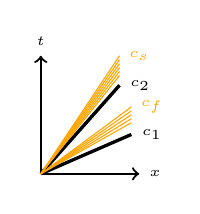
\begin{tikzpicture}[scale=0.5]
                \draw[thick,->] (-0.,0) -- (2.5,0) node[right] {\tiny $x$};
                \draw[thick,->] (-0.,-0.) -- (0,3) node[above] {\tiny $t$};
                \draw[very thick] (0,0) -- (2.3,1.) node[right] {\tiny $c_1$};
                % \draw[very thick] (0,0) -- (-2.3,1.) node[left] {\tiny $-c_1$};
                \draw[very thick] (0,0) -- (2.,2.25) node[right] {\tiny $c_2$};
                % \draw[very thick] (0,0) -- (-2.,2.25) node[left] {\tiny $-c_2$};
                \foreach \x in {1.3,1.4,1.5,1.6,1.7}
                {\draw[Orange] (0,0)-- (2.3,\x);
                  % \draw[Orange] (0,0)-- (-2.3,\x);
                }
                \node[Orange,right] at (2.3,1.7) {\tiny $c_f$};
                % \node[Orange,left] at (-2.3,1.7) {\tiny $-c_f$};
                \foreach \x in {2.5,2.6,2.7,2.8,2.9,3.}
                {\draw[Orange] (0,0)-- (2,\x);
                  % \draw[Orange] (0,0)-- (-2,\x);
                }
                \node[Orange,right] at (2,3) {\tiny $c_s$};
                % \node[Orange,left] at (-2,3) {\tiny $-c_s$};
              \end{tikzpicture}
            \end{column}
            \begin{column}{0.7\textwidth}
              \begin{itemize}
              \item[] fast and slow simple waves: $c_f,c_s$
              \item[] combined-stress waves
              \end{itemize}
            \end{column}
          \end{columns}
        \end{block}
      \end{footnotesize}
    \end{column}
  \end{columns}
  % Governing equations based on elastic-plastic softenesses
  \footnoteCite{CRISTESCU19591605,Rakhmatulin}
\end{frame}


\begin{frame}{Thin-walled tube problem: characteristic analysis \cite{Clifton}}
  \nocite{Clifton}
  \begin{footnotesize}
    \begin{columns}
      \begin{column}{0.6\textwidth}
        \begin{itemize}
          % \item ODEs governing the evolution of stress and velocity through both simple waves
        \item[] ODEs through simple waves: $d\tau=\psi(\tens{\sigma})d\sigma \rightarrow$ loading paths 
          \begin{itemize}
          \item \footnotesize characteristic structure not known a priori%integration: loading paths
          \item \footnotesize mathematical study $\rightarrow$ solution of Picard's problem
            % \centering
            \begin{tikzpicture}
              \draw[->] (0,0) -- (2,0) node[right] {\tiny $x$};
              \draw[->] (0,0) -- (0,2) node[above] {\tiny $t$};
              \node[right] at (1,0.2) {\tiny $\tens{\sigma}^0$};
              \draw (0,0) -- (2,0.65);
              \foreach \y in {0.65,0.7,...,1.}
              \draw (0,0) -- (2,\y);
              \foreach \y in {1.5,1.55,...,2.}
              \draw (0,0) -- (2,\y);
              \node[left] at (1.25,1.5) {\tiny $\color{Red}\tens{\sigma}^1\color{CNBlue}$};
              \begin{scope}[shift={(2.5,0)}]
                \draw[->] (0,0) -- (2,0) node[right] {\tiny $x$};
                \draw[->] (0,0) -- (0,2) node[above] {\tiny $t$};
                \node[right] at (1,0.2) {\tiny $\tens{\sigma}^0$};
                \draw (0,0) -- (2,0.65);
                \foreach \y in {1.5,1.55,...,2.}
                \draw (0,0) -- (2,\y);
                \node[left] at (1.25,1.5) {\tiny $\color{Orange}\tens{\sigma}^2\color{CNBlue}$};
              \end{scope}
              \begin{scope}[shift={(5,0)}]
                \draw[->] (0,0) -- (2,0) node[right] {\tiny $x$};
                \draw[->] (0,0) -- (0,2) node[above] {\tiny $t$};
                \node[right] at (1,0.2) {\tiny $\tens{\sigma}^0$};
                \draw (0,0) -- (2,0.65);
                \foreach \y in {0.65,0.7,...,1.}
                \draw (0,0) -- (2,\y);
                % \foreach \y in {1.5,1.55,...,2.}
                % \draw (0,0) -- (2,\y);
                \draw (0,0) -- (2,1.5);
                \node[left] at (1.25,1.5) {\tiny $\color{Green}\tens{\sigma}^3\color{CNBlue}$};
              \end{scope}
            \end{tikzpicture}
          \item \footnotesize iterative Riemann solver \cite{Lin_et_Ballman}
          \end{itemize}
        \end{itemize}
      \end{column}
      \begin{column}{0.43\textwidth}
        \begin{overprint}
          \onslide<1>
          \vskip 5pt
          \centering
          \begin{tikzpicture}[scale=0.9]
  \begin{axis}[ymajorgrids=true,xmajorgrids=true,ylabel=$\sigma_{12}$,xlabel=$\sigma_{11}$,xmax=2.e8]
    %%
    \addplot[Green,mark=x,only marks,mark repeat=15,very thick] table [x=sigma_11,y=sigma_12] {chapter5/pgfFigures/pgf_thinWalledTubeSlowWave/slowStressPlane_Stress0.pgf};
    \addplot[Green,thick] table [x=sigma_11,y=sigma_12] {chapter5/pgfFigures/pgf_thinWalledTubeSlowWave/TWslowStressPlane_Stress0.pgf};
    %%
    \addplot[Duck,mark=x,only marks,mark repeat=15,very thick] table [x=sigma_11,y=sigma_12] {chapter5/pgfFigures/pgf_thinWalledTubeSlowWave/slowStressPlane_Stress1.pgf};
    \addplot[Duck,thick] table [x=sigma_11,y=sigma_12] {chapter5/pgfFigures/pgf_thinWalledTubeSlowWave/TWslowStressPlane_Stress1.pgf};
    %%
    \addplot[Red,mark=x,only marks,mark repeat=15,very thick] table [x=sigma_11,y=sigma_12] {chapter5/pgfFigures/pgf_thinWalledTubeSlowWave/slowStressPlane_Stress2.pgf};
    \addplot[Red,thick] table [x=sigma_11,y=sigma_12] {chapter5/pgfFigures/pgf_thinWalledTubeSlowWave/TWslowStressPlane_Stress2.pgf};
    %%
    \addplot[Purple,mark=x,only marks,mark repeat=15,very thick] table [x=sigma_11,y=sigma_12] {chapter5/pgfFigures/pgf_thinWalledTubeSlowWave/slowStressPlane_Stress3.pgf};
    \addplot[Purple,thick] table [x=sigma_11,y=sigma_12] {chapter5/pgfFigures/pgf_thinWalledTubeSlowWave/TWslowStressPlane_Stress3.pgf};
    %%
    \addplot[Blue,mark=x,only marks,mark repeat=15,very thick] table [x=sigma_11,y=sigma_12] {chapter5/pgfFigures/pgf_thinWalledTubeSlowWave/slowStressPlane_Stress4.pgf};
    \addplot[Blue,thick] table [x=sigma_11,y=sigma_12] {chapter5/pgfFigures/pgf_thinWalledTubeSlowWave/TWslowStressPlane_Stress4.pgf};
    %%
    \addplot[Orange,mark=x,only marks,mark repeat=15,very thick] table [x=sigma_11,y=sigma_12] {chapter5/pgfFigures/pgf_thinWalledTubeSlowWave/slowStressPlane_Stress5.pgf};
    \addplot[Orange,thick] table [x=sigma_11,y=sigma_12] {chapter5/pgfFigures/pgf_thinWalledTubeSlowWave/TWslowStressPlane_Stress5.pgf};
    %%
    \addplot[Yellow,mark=x,only marks,mark repeat=5,very thick] table [x=sigma_11,y=sigma_12] {chapter5/pgfFigures/pgf_thinWalledTubeSlowWave/slowStressPlane_Stress6.pgf};
    \addplot[Yellow,thick] table [x=sigma_11,y=sigma_12] {chapter5/pgfFigures/pgf_thinWalledTubeSlowWave/TWslowStressPlane_Stress6.pgf};
    %% Yield surface
    \addplot[black,dashed] table  [x=sigma_11,y=sigma_12] {chapter5/pgfFigures/pgf_thinWalledTubeSlowWave/TWslow_yield0.pgf};
  \end{axis}
\end{tikzpicture}

%%% Local Variables:
%%% mode: latex
%%% TeX-master: "../../mainManuscript"
%%% End:
          \onslide<2>
          \vskip 5pt
          \centering
          \begin{tikzpicture}[scale=0.7]
  \begin{axis}[ymajorgrids=true,xmajorgrids=true,ylabel=$\tau \: (Pa)$,xlabel=$\sigma \: (Pa)$,xmin=-0.1e8,xmax=1.5e8,ymin=0.,ymax=7.5e7, legend pos=north east]
    %% Yield surface
    \addplot[black,densely dotted] table  [x=sigma_11,y=sigma_12] {section5/pgfFigures/pgf_thinWalledTubeSlowWave/TWslow_yield0.pgf};
    \addlegendentry{yield surface}
    %%
    \addplot[black,loosely dashed,thick] table  [x=sigma_11,y=sigma_12] {section5/pgfFigures/pgf_thinWalledTubeSlowWave/TWslow_yield0.pgf};
    \addlegendentry{fast wave}
    %% 
    \addplot[very thick] table [x=sigma_11,y=sigma_12] {section5/pgfFigures/pgf_thinWalledTubeSlowWave/TWslowStressPlane_Stress0.pgf};
    \addlegendentry{slow wave}
    %%
    \addplot[very thick] table [x=sigma_11,y=sigma_12] {section5/pgfFigures/pgf_thinWalledTubeSlowWave/TWslowStressPlane_Stress1.pgf};
    %%
    \addplot[very thick] table [x=sigma_11,y=sigma_12] {section5/pgfFigures/pgf_thinWalledTubeSlowWave/TWslowStressPlane_Stress2.pgf};
    %%
    \addplot[very thick] table [x=sigma_11,y=sigma_12] {section5/pgfFigures/pgf_thinWalledTubeSlowWave/TWslowStressPlane_Stress3.pgf};
    %%
    \addplot[very thick] table [x=sigma_11,y=sigma_12] {section5/pgfFigures/pgf_thinWalledTubeSlowWave/TWslowStressPlane_Stress4.pgf};
    %%
    \addplot[very thick] table [x=sigma_11,y=sigma_12] {section5/pgfFigures/pgf_thinWalledTubeSlowWave/TWslowStressPlane_Stress5.pgf};
    %%
    \addplot[very thick] table [x=sigma_11,y=sigma_12] {section5/pgfFigures/pgf_thinWalledTubeSlowWave/TWslowStressPlane_Stress6.pgf};
    %% Yield surface
    \addplot[black,dashed] table  [x=sigma_11,y=sigma_12] {section5/pgfFigures/pgf_thinWalledTubeSlowWave/TWslow_yield0.pgf};

    \addplot[very thick,Red,restrict x to domain=0.2e8:0.5e8] table [x=sigma_11,y=sigma_12]{section5/pgfFigures/pgf_thinWalledTubeSlowWave/TWslow_yield0.pgf};
    \addplot[very thick,Red,restrict y to domain=4.e7:6.5e7] table [x=sigma_11,y=sigma_12] {section5/pgfFigures/pgf_thinWalledTubeSlowWave/TWslowStressPlane_Stress2.pgf};

    \node[right] at (axis cs:0.55e8,6.5e7) {$\color{Red}\tens{\sigma}^1$};
  \end{axis}
\end{tikzpicture}

%%% Local Variables:
%%% mode: latex
%%% TeX-master: "../../presentation"
%%% End:
          \onslide<3>
          \vskip 5pt
          \centering
          \begin{tikzpicture}[scale=0.7]
  \begin{axis}[ymajorgrids=true,xmajorgrids=true,ylabel=$\tau \: (Pa)$,xlabel=$\sigma \: (Pa)$,xmin=-0.1e8,xmax=1.5e8,ymin=0.,ymax=7.5e7, legend pos=north east]
    %% Yield surface
    \addplot[black,densely dotted] table  [x=sigma_11,y=sigma_12] {section5/pgfFigures/pgf_thinWalledTubeSlowWave/TWslow_yield0.pgf};
    \addlegendentry{yield surface}
    %%
    \addplot[black,loosely dashed,thick] table  [x=sigma_11,y=sigma_12] {section5/pgfFigures/pgf_thinWalledTubeSlowWave/TWslow_yield0.pgf};
    \addlegendentry{fast wave}
    %% 
    \addplot[very thick] table [x=sigma_11,y=sigma_12] {section5/pgfFigures/pgf_thinWalledTubeSlowWave/TWslowStressPlane_Stress0.pgf};
    \addlegendentry{slow wave}
    %%
    \addplot[very thick] table [x=sigma_11,y=sigma_12] {section5/pgfFigures/pgf_thinWalledTubeSlowWave/TWslowStressPlane_Stress1.pgf};
    %%
    \addplot[very thick] table [x=sigma_11,y=sigma_12] {section5/pgfFigures/pgf_thinWalledTubeSlowWave/TWslowStressPlane_Stress2.pgf};
    %%
    \addplot[very thick] table [x=sigma_11,y=sigma_12] {section5/pgfFigures/pgf_thinWalledTubeSlowWave/TWslowStressPlane_Stress3.pgf};
    %%
    \addplot[very thick] table [x=sigma_11,y=sigma_12] {section5/pgfFigures/pgf_thinWalledTubeSlowWave/TWslowStressPlane_Stress4.pgf};
    %%
    \addplot[very thick] table [x=sigma_11,y=sigma_12] {section5/pgfFigures/pgf_thinWalledTubeSlowWave/TWslowStressPlane_Stress5.pgf};
    %%
    \addplot[very thick] table [x=sigma_11,y=sigma_12] {section5/pgfFigures/pgf_thinWalledTubeSlowWave/TWslowStressPlane_Stress6.pgf};
    %% Yield surface
    %\addplot[black,dashed] table  [x=sigma_11,y=sigma_12] {section5/pgfFigures/pgf_thinWalledTubeSlowWave/TWslow_yield0.pgf};

    
    \addplot[very thick,Orange,restrict y to domain=4.e7:6.75e7] table [x=sigma_11,y=sigma_12]{section5/pgfFigures/pgf_thinWalledTubeSlowWave/TWslowStressPlane_Stress1.pgf};
    \addplot[very thick,Orange,arrows along my path] coordinates{(0.25e8,5.6e7) (0.25e8,0.) (0,0)};
    
    \node[right] at (axis cs:0.25e8,6.75e7) {$\color{Orange}\tens{\sigma}^2$};
  \end{axis}
\end{tikzpicture}

%%% Local Variables:
%%% mode: latex
%%% TeX-master: "../../presentation"
%%% End:
          \onslide<4>
          \vskip 5pt
          \centering
          \begin{tikzpicture}[scale=0.7]
  \begin{axis}[ymajorgrids=true,xmajorgrids=true,ylabel=$\tau \: (Pa)$,xlabel=$\sigma \: (Pa)$,xmin=-0.1e8,xmax=1.5e8,ymin=0.,ymax=7.5e7, legend pos=north east]
    %% Yield surface
    \addplot[black,densely dotted] table  [x=sigma_11,y=sigma_12] {section5/pgfFigures/pgf_thinWalledTubeSlowWave/TWslow_yield0.pgf};
    \addlegendentry{yield surface}
    %%
    \addplot[black,loosely dashed,thick] table  [x=sigma_11,y=sigma_12] {section5/pgfFigures/pgf_thinWalledTubeSlowWave/TWslow_yield0.pgf};
    \addlegendentry{fast wave}
    %%
    \addplot[very thick] table [x=sigma_11,y=sigma_12] {section5/pgfFigures/pgf_thinWalledTubeSlowWave/TWslowStressPlane_Stress0.pgf};
    \addlegendentry{slow wave}
    %%
    \addplot[very thick] table [x=sigma_11,y=sigma_12] {section5/pgfFigures/pgf_thinWalledTubeSlowWave/TWslowStressPlane_Stress1.pgf};
    %%
    \addplot[very thick] table [x=sigma_11,y=sigma_12] {section5/pgfFigures/pgf_thinWalledTubeSlowWave/TWslowStressPlane_Stress2.pgf};
    %%
    \addplot[very thick] table [x=sigma_11,y=sigma_12] {section5/pgfFigures/pgf_thinWalledTubeSlowWave/TWslowStressPlane_Stress3.pgf};
    %%
    \addplot[very thick] table [x=sigma_11,y=sigma_12] {section5/pgfFigures/pgf_thinWalledTubeSlowWave/TWslowStressPlane_Stress4.pgf};
    %%
    \addplot[very thick] table [x=sigma_11,y=sigma_12] {section5/pgfFigures/pgf_thinWalledTubeSlowWave/TWslowStressPlane_Stress5.pgf};
    %%
    \addplot[very thick] table [x=sigma_11,y=sigma_12] {section5/pgfFigures/pgf_thinWalledTubeSlowWave/TWslowStressPlane_Stress6.pgf};
    %% Yield surface
    \addplot[black,dashed] table  [x=sigma_11,y=sigma_12] {section5/pgfFigures/pgf_thinWalledTubeSlowWave/TWslow_yield0.pgf};

    \addplot[very thick,Green,restrict x to domain=0.4e8:0.95e8,arrows along my path] table [x=sigma_11,y=sigma_12]{section5/pgfFigures/pgf_thinWalledTubeSlowWave/TWslow_yield0.pgf};

    \addplot[very thick,Green,arrows along my path] coordinates{(0.42e8,5.25e7) (0.42e8,0.) (0,0)  };
    
    \node[right] at (axis cs:0.95e8,1.8e7) {$\color{Green}\tens{\sigma}^2$};
  \end{axis}
\end{tikzpicture}

%%% Local Variables:
%%% mode: latex
%%% TeX-master: "../../presentation"
%%% End:
          
        \end{overprint}
        
      \end{column}
    \end{columns}
  \end{footnotesize}
  % \cite{Clifton,Clifton_exp}
  \footnoteCite{Clifton,Lin_et_Ballman}
\end{frame}

\subsection{General formulation}
\begin{frame}
  \begin{block}{Problems tackled overall}
    \begin{itemize}
    \item Particular plane strain and plane stress cases \cite{Bleich,Ting69,Ting73,Li_planeStress_EP}
    \item Equations based on elastic-plastic compliances
    
    \end{itemize}
  \end{block}
  \begin{block}{The proposed approach}
    Hyperbolic system in the arbitrary direction $\vect{n}$: $\drond{\Qcb}{t} + \Jbsf \drond{\Qcb}{x_n} =\vect{0}$ \\
    $\Jbsf=-\matrice{\tens{0}^2 & \frac{1}{\rho}\tens{I}\otimes\vect{n} \\ \alert{\Cbb^{ep}\cdot \vect{n}} & \tens{0}^4}$
    \begin{itemize}
    \item General plane strain and plane stress problems \textbf{under small strains}
    \item Unified framework
    % \item generalizes to plane strain and plane stress problems
    \end{itemize}
  \end{block}
  \footnoteCite{Bleich,Ting69,Ting73,Li_planeStress_EP}
\end{frame}

% \begin{frame}
  % \begin{block}{Governing equations}
  %   \begin{footnotesize}
  %     \begin{columns}
  %       \begin{column}{0.4\textwidth}
  %         \begin{flalign*}
  %           & \text{plastic flow: } \dot{\tens{\eps}}^p = \dot{p}\drond{f}{\tens{\sigma}} \\
  %           & \text{constitutive equations: } \dot{\tens{\sigma}}=\Cbb^{ep}:\dot{\tens{\eps}} \\
  %           & \text{linear momentum: } \drond{\rho \vect{v}}{t} - \nabla_v \cdot\tens{\sigma} = \vect{0}\\
  %           & \text{kinematic laws: } \dot{\tens{\eps}} = \nablat^s \vect{v}
  %         \end{flalign*}
  %       \end{column}
  %       \begin{column}{0.55\textwidth}
  %         \begin{flalign*}
  %           \Rightarrow \: &\text{quasi-linear form: } \drond{\Ucb}{\Qcb}\drond{\Qcb}{t} + \drond{\Fcb\cdot\vect{e}_i}{\Qcb}\drond{\Qcb}{x_i}=\vect{0} \\
  %           & \Ucb = \matrice{\rho \vect{v} \\ \tens{\eps}} \: ; \: \Qcb = \matrice{\vect{v} \\ \tens{\sigma}} \: ;\: \Fcb \cdot \vect{e}_i = -\matrice{\sigma_{ji}  \\ \frac{v_j \delta_{ik} + v_i \delta_{jk}}{2}}, (i,j,k) = \{1,2,3\}
  %         \end{flalign*}
  %       \end{column}
  %     \end{columns}
  %     %Difference with previous formulations ? Inverse $\drond{\Ucb}{\Qcb}$ rather than its matrix representation $\rightarrow$ stiffnesses instead of softenesses
  %     %% system kept generical so far
  %   \end{footnotesize}
  %   \begin{block}{Hyperbolic system in the arbitrary direction $\vect{n}$}
  %     \begin{flalign*}
  %       \drond{\Qcb}{t} + \Jbsf \drond{\Qcb}{x_n} =\vect{0}
  %     \end{flalign*}
  %     with the Jacobian matrix $\Jbsf=-\matrice{\tens{0}^2 & \frac{1}{\rho}\tens{I}\otimes\vect{n} \\ \alert{\Cbb^{ep}\cdot \vect{n}} & \tens{0}^4}$
  %   \end{block}
  % \end{block}
% \end{frame}



%%% Local Variables:
%%% mode: latex
%%% TeX-master: "../presentation"
%%% End:
